\documentclass[12pt,a4paper]{article}
\usepackage[utf8]{inputenc}
\usepackage[T1]{fontenc}
\usepackage[english, swedish]{babel}
\usepackage{amsmath}
\usepackage{ae}
\usepackage{units}
\usepackage{icomma}
\usepackage{color}
\usepackage{graphicx}
\usepackage{bbm}
\usepackage{textcomp}
\usepackage{url}
\usepackage{verbatim}
\usepackage{subfig}
\usepackage{marvosym}
\usepackage{eso-pic}
\usepackage[margin=0.5in]{geometry}

\newcommand{\N}{\ensuremath{\mathbbm{N}}}
\newcommand{\Z}{\ensuremath{\mathbbm{Z}}}
\newcommand{\Q}{\ensuremath{\mathbbm{Q}}}
\newcommand{\R}{\ensuremath{\mathbbm{R}}}
\newcommand{\C}{\ensuremath{\mathbbm{C}}}
\usepackage{amssymb}
\newcommand{\rd}{\ensuremath{\mathrm{d}}}
\newcommand{\id}{\ensuremath{\,\rd}}
\linespread{1.3}
%\setcounter{secnumdepth}{-1}

\newcommand\BackgroundPic{
\put(-4,0){
\parbox[b][\paperheight]{\paperwidth}{

\includegraphics[width=\paperwidth,
keepaspectratio]{logga.png}
\vfill
}}}

\begin{document}
\AddToShipoutPicture*{\BackgroundPic}
\begin{titlepage}

%%\Huge{\textbf{CHALMERS}}

\flushleft
\mbox{}
\vspace{7cm}

\begin{center}

\Large{Planeringsrapport}

\Huge{\textbf{Stabilisera temperaturen i en fastighet \\ med avseende på väderförändringar}}

\end{center}

\vspace{2cm}
\begin{table}[h!]
\begin{center}
\begin{tabular}{ c c }
\textbf{Erik Ahlqvist} \hspace{1cm} & \textbf{Mats Lindström} \\ 
\footnotesize{erikahl@student.chalmers.se} \hspace{1cm} & \footnotesize{limats@student.chalmers.se} \vspace{0.5cm} \\ 
\textbf{Ylva Dahl} \hspace{1cm} & \textbf{Dan Ståby} \\
\footnotesize{ylvad@student.chalmers.se} \hspace{1cm} & \footnotesize{staby@student.chalmers.se} \\
\end{tabular}
\end{center}
\end{table}

\vfill

Institutionen för Teknisk Fysik \hfill Handledare:\\
CHALMERS TEKNISKA HÖGSKOLA \hfill Magnus Karlsteen\\
Göteborg, Sverige, \today \hfill Peter Särneö\\

\end{titlepage}

\newpage
\thispagestyle{empty}
\mbox{}
\newgeometry{}

\newpage
\pagenumbering{roman}
\tableofcontents

\newpage
\pagenumbering{arabic}
\setcounter{page}{1}
%\setlength{\parindent}{0pt}
%\setlength{\parskip}{1.5ex plus 0.5ex minus 0.3ex}

\section{Bakgrund}

Energi flödar hela tiden in och ut ur fastigheter, bland annat genom människors kroppsvärme, VVA (värme, ventilation och avlopp) och vädret ute. Dessa energiflöden kan delas in i konstanta energiflöden samt variabla energiflöden. Den främsta variabla energikällan är troligen vädret. Vädret kan, genom sina skiftningar, både ge och ta energi från byggnaden. För att bibehålla en jämn inomhustemperatur i fastigheten kan inte en konstant mängd energi tillföras av värmesystemet, utan energitillförseln måste hela tiden regleras utefter både konstanta samt variabla energiflöden.

I dagsläget regleras de flesta energisystem i fastigheter endast med tanke på utomhustemperaturen i varje ögonblick och på så sätt blir det alltid en fördröjning i uppvärmningen vilket i vårt fall leder till ojämn inomhustemperatur och eventuellt också till onödig energiåtgång.

Vår uppdragsgivare sköter utrustning för uppvärmning av fastigheten. Han har ett pågående projekt med syfte att minska energiförbrukningen i fastigheten samtidigt som ett behagligt inomhusklimat bibehålls. Inom ramen för detta så har en väderstation installerats på taket till fastigheten och sensorer av diverse slag har anslutits på strategiska platser.  Dessa enheter tillåter uppvärmningssystemet att anpassa energianvändningen efter väderlek.

Denna typ av effektivisering av energianvändningen i en fastighet är idag högaktuell på grund av höga energipriser och ökad förståelse för hur vår energianvändning kan påverka planeten negativt.

\section{Syfte}

I detta arbete ska vi undersöka vilka energiförluster vi har i en fastighet och hur dessa påverkas av olika väderrelaterade parametrar.

Vi vill finna en modell som visar på hur fastighetens energiflöde ska regleras med avseende på de opåverkbara men föränderliga energiflöden som sker in och ut i fastigheten, till exempel på grund av väder, så att ett önskat inomhusklimat bibehålls. Vi avser då också att ta hänsyn till den fördröjning som sker i och med fastighetens relativt tjocka väggar. Mer konkret söker vi en ekvation som ger oss ett värde på hur mycket energi som behöver tillföras fastigheten i varje givet ögonblick, beroende på vilka värden väderstationen tidigare har tagit emot.

Vi hoppas också att detta ska ge, inte bara en trivsammare inomhusmiljö för de boende, utan även en energibesparing för fastigheten.

\section{Problem}

Många moderna värmesystem är programmerade enligt vissa konstanta egenskaper hos huset, som byggnadsmaterial, storlek, isolering samt i vissa fall hur mycket värme som tillförs genom antalet boende och värmeproducerande apparatur. Den enda variabeln som tas hänsyn till är därefter utetemperaturen. Uppvärmningen regleras alltså varken efter husets eller värmesystemets tröghet, eller någon annan väderfaktor.

Ett första steg i vårt arbete blir att ta fram ett energiflödesschema för fastigheten där alla konstanta flöden kan identifieras. Sådana kan till exempel vara cirkulerande varmvatten för hushållsbruk, värmeproducerande vitvaror samt kroppsvärme från människor. Denna energi kan inte påverkas på samma sätt som radiatorvärmen och bör kunna sättas konstant. Genom att identifiera alla dess källor kan vi också finna ett värde för den.

Nästa steg blir att utöka energiflödesschemat med de väderparametrar\footnote{Temperatur, nedebörd, vindriktning, vindfart, luftfuktighet, lufttryck, solintensitet.} som kan mätas med väderstationen som finns monterad på fastighetens tak. Dessa ger eller tar energi från fastigheten och kan inte heller påverkas. De är dock variabla och kräver därför att man närmare studerar hur de påverkar fastighetens temperatur. Två begrepp som vi då har till vår hjälp är oreglerad (free-running) temperatur – temperatur i lägenheten utan radiatoruppvärmning samt ekvivalent temperatur – alla väderparametrar sammanlagda.

Genom att veta hur mycket energi som går in och ut ur huset i kombination med väderdata och kunskap om trögheten i väggarna kan vi beräkna hur mycket energi som behöver tillföras för att en behaglig boendetemperatur ska kunna uppnås. På grund av just fördöjningen i väggar och tak vet vi helt säkert vilket väder vi ska räkna med, för när vi väl ska reglera för värdet har det redan hänt. Vi söker en oreglerad (free-running) temperatur med vilken vi kan bestämma hur stort energiinflöde som behövs i varje ögonblick. Detta ger oss möjlighet att ta fram en modell för styrsystemet. Vi kommer här att se på fastigheten som en enhet med en temperatur.

Vi hoppas att vi kan få data från fastigheten för att även kunna göra statistiska modeller och jämföra dem med våra teoretiska resultat. Finns inte den möjligheten vill vi ändå ta fram förslag på hur statistisk data kan behandlas när det väl finns tillgång till den. Utifrån dessa modeller bör det även gå att beräkna en approximativ siffra på energibesparingen vid infört system.

Som en sista del avser vi att undersöka hur reglersystemet ska byggas upp då man har termometrar i varje rum och hur systemet skulle kunna göras självförbättrande.

\section{Avgränsningar}

En detaljerad specifikation av värmeanläggningen och instruktioner för hur den ska drivas för att optimera energiförbrukningen kommer inte att ges i denna rapport, eftersom detta för sig självt skulle kunna omfattas av ett eget kandidatarbete. Baserat på resultatet av detta arbete ska man däremot kunna bygga vidare mot en sådan tillämpning, med exempelvis dimensionering av ett reglersystem som följd.

Om jämförelser med empiriska resultat kommer vara möjliga är i nuläget osäkert. Det beror på i vilken grad vi får tillgång till data från väderstationen, men också på om vi kommer kunna använda oss av data från utomstående part. Det skulle vara möjligt att jämföra data från väderstationen med väderprognoser från SMHI eller motsvarande. Utifrån detta kommer vi att analysera fördelarna med att använda prognosstyrning.

Vi kommer att bortse från snabba temperaturfluktuationer orsakade av exempelvis öppna fönster eller värmeeffekten från onormalt många människor i lägenheterna. Dessa är svåra, om inte omöjliga, att förutse.

\section{Metod}

Till att börja med skall vi utföra en litteraturstudie för att se relevant forskning på området energiförluster i en byggnad. Detta för att ge oss banor att fundera i när vi fortsätter att räkna på byggnaden teoretiskt. Teoretisk beräkning kan genomföras genom att till exempel sätta upp en datormodell med de relevanta differentialekvationerna samt parametrarna och approximera lösningen till dessa med exempelvis finita elementmetoden. Här planerar vi att beräkna värmeflöden från de olika väggarna, från taket, från fönster samt från grunden av byggnaden. Vi skall också beräkna hur dessa flöden påverkas av olika väderrelaterade parametrar. Här kan vi säkert få en del hjälp från det tidigare kandidatarbete som behandlat byggnaden.

De framräknade värdena kan med fördel jämföras med empiriska data. Förhoppningsvis kommer vår uppdragsgivare att tillhandahålla oss med mätdata från den i fastigheten installerade mätutrustningen. Dessa data kan även användas för att se hur inomhustemperaturer kovarierar med väder. Denna typ av analys är högintressant för att bygga ett smart självanpassande system som styr inomhusklimatet.

För att se om det finns några defekter på byggnaden som läcker särskilt mycket värme så planerar vi att fotografera byggnaden med hjälp av en värmekamera och på så sätt ha möjlighet att se var de största förlusterna ligger eller om vi har homogena värmeförluster från väggarna.

När vi har fastställt en god modell för hur väder och vind påverkar fastighetens energiflöden så bör vi analysera hur stor energibesparing som kan genomföras genom att ta hänsyn till dessa parametrar i jämförelse med dagens utformning av reglersystem. Här bör vi även ha skapat ett diagram som visar alla värmeflöden in och ut ur fastigheten. Detta kan vara ett gott hjälpmedel för uppdragsgivaren för att fortsätta med det pågående energibesparingsprojektet.

\restoregeometry

\section[Tidsplan]{Tidsplan\footnote{Gantt-schemat finns även interaktivt via Google Dokument, delat internt inom gruppen}}

\begin{figure}[h!]\centering
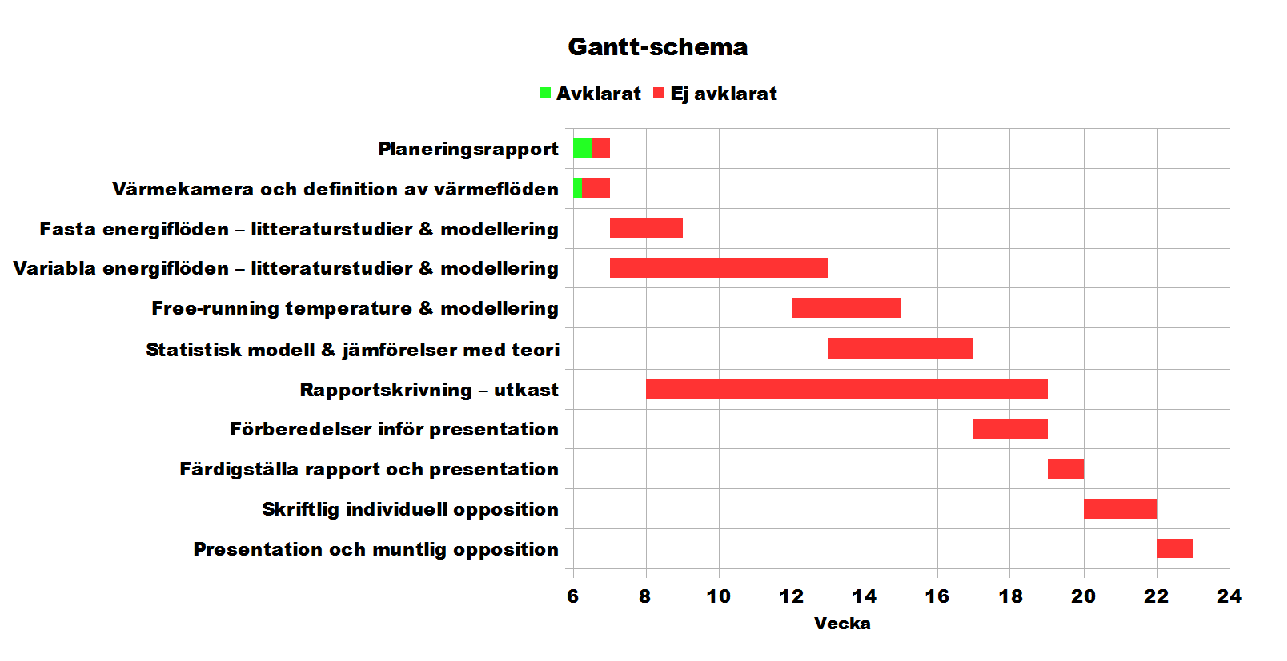
\includegraphics[scale=0.7, angle=270]{Gantt.png}
\end{figure}

% Tabell
%%\begin{table}[h!]
%%\begin{center}
%% \begin{tabular}{ l | c || r | }
%%   \hline
%%    1 & 2 & 3 \\ \hline
%%    4 & 5 & 6 \\ \hline
%%    7 & 8 & 9 \\
%%    \hline
%%  \end{tabular}
%%\caption{}
%%\end{center}
%%\end{table}

\end{document}
